\documentclass{article}
\usepackage{graphicx}
\usepackage{listings}
\usepackage{color}

\title{TCP File Transfer Protocol Report}
\author{Jackie Chan}
\date{\today}

\begin{document}
	
	\maketitle
	
	\section{Protocol Design}
	The file transfer protocol was designed as a simple client-server model using TCP/IP sockets. The protocol involves establishing a connection, transferring data in chunks, and handling errors effectively.
	
	\begin{figure}[h]
		\centering
		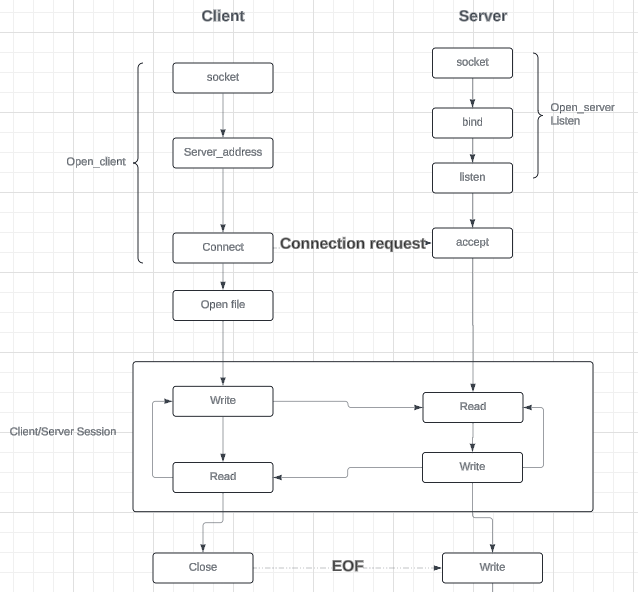
\includegraphics[width=0.6\textwidth]{DesigeSystem.png}
		\caption{Protocol Design Overview}
	\end{figure}
	
	When running the program. We run the server first to create the server. Then run the client. Note, the client's code must match the server's PORT. The client finds the server's address and starts reading the file to be transferred. The file is read and written by the Client to the Server, and the server will also read and rewrite the data of that file to another file created by the server. After the data is transferred to the server, close the opened methods such as reading/writing files, and close the server.
	
	\section{System Organization}
	The system is organized with a client-server architecture. The client initiates a connection to the server and sends the file in chunks. The server receives the data and saves it to a file.
	
	\begin{minipage}{0.6\textwidth}
		The Server is responsible for receiving files and backing them up from the Client. Step 1, the Server is initialized from the socket, setting the PORT address and linking the socket to the PORT using bin. Then the Server is in Listen mode, ready to receive information from the Client. Next, accept connections from the Client. The steps to create the Server are all placed in the conditional function to control errors. Finally, the Server receives information sent from the Client using int data, and converts the int data to text and saves it to the installed Server file. After saving the data, the Server closes the connection and closes the socket.
	\end{minipage}%
	\begin{minipage}{0.4\textwidth}
		\begin{flushright}
			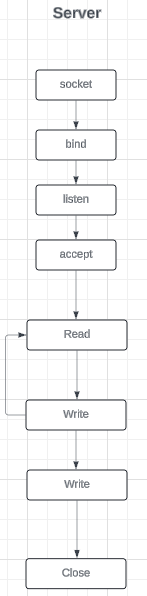
\includegraphics[width=0.8\textwidth, height = 8cm]{OragnizeSystemServer.png}
			\caption{System Organization in Server}
		\end{flushright}
	\end{minipage}

\begin{figure}[h]
	\centering
	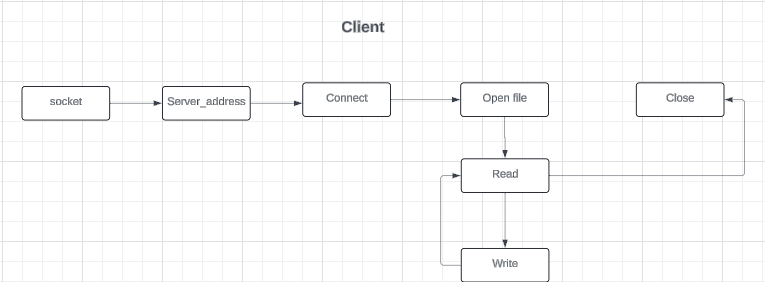
\includegraphics[width=0.8\textwidth]{OragnizeSystemClient.png}
	\caption{System Organization in Client}Client
\end{figure}
	
	The Client is responsible for sending the available file to the server, through the socket. First, the Client will create a socket and then connect to the server through the server's PORT which is pre-defined in the code. The process of connecting to the Server is placed in a conditional function to detect errors in any part of the system. After the Client connects to the Server, the Client will open the file and read the data in the file, then convert it to int format and write to the Server. After the Client has read all the data, the Client closes the file reading and socket functions.
	
	\section{File Transfer Implementation}
	Below is a code snippet illustrating the implementation of the file transfer protocol:
	
	
	\begin{lstlisting}[language=C, caption=Server file in C]
		#include <stdio.h>
		#include <stdlib.h>
		#include <string.h>
		#include <sys/socket.h>
		#include <sys/types.h>
		#include <netinet/in.h>
		#include <unistd.h>
		
		#define PORT 1402
		
		int main() {
			int server_fd, new_socket;
			struct sockaddr_in address;;
			int addrlen = sizeof(address);
			char buffer[1024] = {0};
			FILE *received_file;
			char *file_name= "received.txt";
			
			if ((server_fd = socket(AF_INET, SOCK_STREAM, 0)) == 0) {
				perror("socket creation failed");
				exit(EXIT_FAILURE);
			}
			
			address.sin_family = AF_INET;
			address.sin_addr.s_addr = INADDR_ANY;
			address.sin_port = htons(PORT);
			
			if (bind(server_fd, (struct sockaddr *)&address, addrlen) < 0) {
				perror("bind failed");
				exit(EXIT_FAILURE);
			}
			
			if (listen(server_fd, 5) < 0) {
				perror("listen failed" );
				exit(EXIT_FAILURE);
			}
			if ((new_socket = accept(server_fd, (struct sockaddr *)&address, (socklen_t*)&addrlen)) < 0) {
				perror("accept failed");
				exit(EXIT_FAILURE);
			}
			
			received_file = fopen("received.txt", "wb");
			while (1) {
				int bytes_read = read(new_socket, buffer, 1024);
				if (bytes_read <= 0) {
					break;
				}
				fwrite(buffer, 1, bytes_read, received_file);
			}
			
			printf("File recevived successfully.\n");
			fclose(received_file);
			close(new_socket);
			close(server_fd);
			return 0;
			
		}
		
		//
		// Created by jackiechan on 11/23/24.
		//
		
	\end{lstlisting}

	\begin{lstlisting}[language=C, caption=Client file in C]
		#include <stdio.h>
		#include <stdlib.h>
		#include <string.h>
		#include <sys/types.h>
		#include <sys/socket.h>
		#include <netinet/in.h>
		#include <arpa/inet.h>
		#include <unistd.h>
		
		#define PORT 1402
		#define SERVER_IP "127.0.0.1"
		
		int main() {
			int client_fd;
			struct sockaddr_in server_address;
			char buffer[1024] = {0};
			FILE *file;
			char *filename = "file.txt";
			
			if ((client_fd = socket(AF_INET, SOCK_STREAM, 0)) < 0) {
				perror("socket creation failed");
				exit(EXIT_FAILURE);
			}
			
			server_address.sin_family = AF_INET;
			server_address.sin_port = htons(PORT);
			
			if (inet_pton(AF_INET, SERVER_IP, &server_address.sin_addr) <= 0) {
				perror("Invalid address/ Address not given");
				exit(EXIT_FAILURE);
			}
			
			if (connect(client_fd, (struct sockaddr *)&server_address, sizeof(server_address)) < 0) {
				perror("Connection failed");
				exit(EXIT_FAILURE);
			}
			
			file = fopen(filename, "rb");
			if (file == NULL) {
				perror("Could not open file");
				exit(EXIT_FAILURE);
			}
			
			while (1) {
				int bytes_read = fread(buffer, sizeof(char), 1024, file);
				if (bytes_read <= 0) {
					break;
				}
				write(client_fd, buffer, bytes_read);
			}
			
			printf("File sent successfully\n");
			fclose(file);
			close(client_fd);
			
			return 0;
		}
		
		
		//
		// Created by jackiechan on 11/23/24.
		//
		
		
			\end{lstlisting}
	
\end{document}